\documentclass[openany,11pt,a4paper]{report}

\usepackage{xcolor}
\usepackage{url}
\usepackage{array}
\usepackage{caption}
\usepackage{float}
%\usepackage{times}


\usepackage{amsmath} 
\usepackage{amssymb} 
\usepackage{bm}
\usepackage[colorlinks=true,breaklinks]{hyperref} 
\usepackage[hyphenbreaks]{breakurl} %
\usepackage{xcolor}
\definecolor{c1}{rgb}{0,0,1} % blue
\definecolor{c2}{rgb}{0,0.3,0.9} % light blue
\definecolor{c3}{rgb}{0.3,0,0.9} % red blue
\hypersetup{
linkcolor={c1}, 
citecolor={c2}, 
urlcolor={c3} 
}

\usepackage[nottoc]{tocbibind} 
\usepackage{graphicx}
\usepackage{longtable} 
\usepackage{bigstrut} 
\usepackage{enumerate}
\usepackage{todonotes} 
\usepackage{makeidx} 
\usepackage{color}


\usepackage{blindtext}




\makeindex

\usepackage[top=1.5cm, bottom=1.5cm,left=2.5cm,right=2.5cm]{geometry} % needed for page border settings
\parindent=0cm % for space of first line of new text block
\sloppy % for writing with hyphenless justification (tries to)
\hyphenation{} % use hyphenation of tolerance parameters, http://www.jr-x.de/publikationen/latex/tipps/zeilenumbruch.html
\hyphenpenalty=10000
\exhyphenpenalty=10000
\usepackage{fancyhdr}
%\usepackage[pdftex]{graphicx}



\begin{document}

\pagestyle{empty}


\begin{titlepage}

\newcommand{\HRule}{\rule{\linewidth}{0.5mm}} 
\center 

\textsc{\LARGE University of Bonn}\\[1.5cm]
\textsc{\Large Advanced Lab Course}\\[0.5cm] 

\vfill


\HRule \\[0.4cm]
{\huge \textbf {M2.8 Raman Spectroscopy }}

 
\vfill

\begin{minipage}{0.4\textwidth}
\begin{flushleft} \large
\emph{Group 27}\\
Panagiota \textsc{Kardala}\\
Rabia \textsc{Zahid} 
\end{flushleft}
\end{minipage}
~
\begin{minipage}{0.4\textwidth}
\begin{flushright} \large
\emph{Tutor:} \\
{Raphael German} 
\end{flushright}
\end{minipage}\\[4cm]


\vfill

{\large \today}\\[3cm] 

\vfill

\end{titlepage}



\pagestyle{plain}

\tableofcontents







\begin{abstract}

\end{abstract}


\chapter{Theoretical background}

\section{Introduction}

The Raman effect is the inelastic scattering of light which is similar to the Compton effect. It was first predicted by Smekai in 1923 and then was experimentally proved by Raman in 1928. In this experiment, we had to determine the Raman spectra of single crystalline samples for different directions of the incoming and the scattered light. Raman tensors and the symmetries of the obtained spectrum had to be determined. \cite{bib1}

\subsection*{Lattice vibrations and Phonons}

The ions in a crystal are arranged in  fixed positions in a periodical lattice having a certain potential energy. The energy of the system is increased if the ions are displaced from their positions. According to quantum theory, their is a energy quantum also termed as phonons which separates the excited state from the ground state.  In this case, the displacement of a single ion will cause a change in the other surrounding ions. There are patterns of these displacements and vibrations of these kind are called Eigenmodes of the crystal. They have a certain frequency which depends on the wave vector and on the patterns of displacement.
If we assume N number of ions in a unit cell, then the displacement in x, y and z direction leads to total 3N number of ions. The three acoustic modes as shown in Figure 1.1 depicts the translations of the hole crystal and the number of optical phonons become $3N-3$. \cite{bib1}




\begin{figure}[H]
\centering
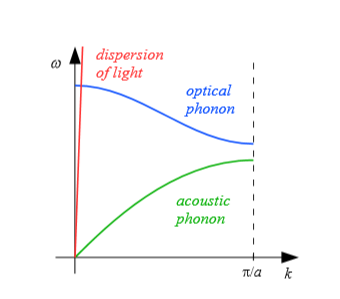
\includegraphics[scale=1]{fig2.PNG}   
\caption{\cite{bib1}}
\end{figure}


\subsection{Raman Spectroscopy}
When a light of single frequency or wavelength with a wavenumber $\bar{\nu_{0}}$ shines on a crystal, some part of it transmits through the material but some of it is scattered away. It is observed, that the scattered radiation consists of an additional wavenumber of the form $\bar{\nu}=\bar{\nu}_{0}+\bar{\nu_{M}}$. At molecular levels the wavenumbers are usually related with the rotational, vibrational and electronic transitions.  
This kind of scattering of light is referred as the Raman Scattering. Raman spectroscopy is one of the most popular techniques to study the structure of molecules.
The additional frequencies in the Raman scattering are because of the energy transfers associated with the system and the incoming radiation. When a radiation of a particular frequency is incident on the system then it is excited from lower energy level $E_{1}$ to a higher energy level $E_{2}$. Where, the energy gap $\Delta E = E_{2}-E_{1}$ is represented by the wavenumber $\bar{\nu_{M}}$. 

\begin{equation}
\Delta E=h c \bar{\nu}_{M}
\end{equation}

This energy gap is the sum of the incident radiation $hc\bar{\nu_{M}}$ and the emitted radiation. The emission of a smaller energy takes place when the scattering of a lower wavenumber occurs. Which is represented by, \begin{equation}
h c\left(\tilde{\nu}_{0}-\tilde{\nu}_{M}\right)
\end{equation}

The interaction of the radiation with the system can also cause another transition  from a high energy level $E_{2}$ to a low energy level $E_{1}$ which is written as,
\begin{equation}
E_{2}-E_{1}=h c \bar{\nu}_{M}
\end{equation}


On the other hand, the emission of a larger energy takes place when the scattering of a higher wavenumber occurs which is given by,
\begin{equation}
h c\left(\tilde{\nu}_{0}+\tilde{\nu}_{M}\right)
\end{equation}
 
Rayleigh scattering takes place when there is no change in the energy of the system after the scattering process. The wavenumber $\tilde{\boldsymbol{\nu}}_{0}$ remains unchanged because  the energy of the emitted photon is same as the one which was absorbed i.e. $h c \tilde{\mathcal{V}}_{0}$.  
 
The Raman band is characterized by the wavenumber shift $\tilde{\nu}_{M}$. This wavenumber shift is also referred as the Raman wavenumbers.  The waveumber shift is positive for Stokes scattering and negative for anti-stokes scattering as represented by Figure 1.1. \cite{bib2}
\begin{figure}[H]
\centering
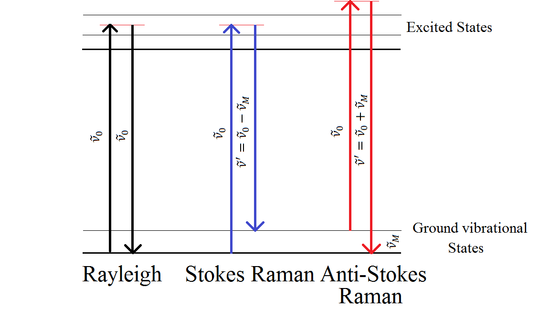
\includegraphics[scale=1]{fig1.png}   
\caption{\cite{bib2}}
\end{figure}

\subsection{Classical Theory}

The electromagnetic radiation theory can be used to explain the scattering phenomena. 

The dipole moment $\mu$ induced by the electric field is usually taken which is represented by power series. 
\begin{equation}
\mu=\mu^{(1)}+\mu^{(2)}+\mu^{(3)}+\cdots
\end{equation}

Where,

\begin{equation}
\begin{aligned} \mu^{(1)} &=\alpha \cdot \mathbf{E} \\ \mu^{(2)} &=\frac{1}{2} \beta \cdot \mathbf{E} \mathbf{E} \\ \mu^{(3)} &=\frac{1}{6} \gamma \cdot \mathbf{E} \mathbf{E} \mathbf{E} \end{aligned}
\end{equation}

Here, $\alpha$ is the polarizability tensor with magnitude 
$10^{-40} \mathrm{cv}^{-1} \mathrm{m}^{2}$, $\beta$ is $10^{-50} \mathrm{CV}^{-2} \mathrm{m}^{3}$ and $\gamma$ is $10^{-61} \mathrm{cv}^{-3} \mathrm{m}^{4}$. Rayleigh and Raman scattering are observed with low electric field intensities which is why it is usually explained by $\mu^{(1)}$ because $\mu^{(2)}$ and $\mu^{(3)}$ are very small for small electric field intensities.

The polarizability tensor for the interaction of a molecular system with the harmonically oscillating electric field is expressed by Taylor series,

\begin{equation}
\alpha_{i j}=\left(\alpha_{i j}\right)_{0}+\sum_{k}\left(\frac{\partial \alpha_{i j}}{\partial Q_{k}}\right)_{0} Q_{k}+\frac{1}{2} \sum_{k, l}\left(\frac{\partial^{2} \alpha_{i j}}{\partial Q_{k} \partial Q_{l}}\right)_{0} Q_{k} Q_{l}+\cdots
\end{equation}

Where, $\left(a_{i j}\right)_{0}$ is the $a_{i j}$ value at equilibrium and $Q_{k}$ and  $Q_{l}$ are normal coordinates. Now, for one normal mode,
\begin{equation}
\alpha_{i j}=\left(\alpha_{i j}\right)_{0}+\left(\frac{\partial \alpha_{i j}}{\partial Q_{k}}\right)_{0} Q_{k}
\end{equation}

For harmonic vibration,

\begin{equation}
Q_{k}=Q_{k 0} \cos \left(\omega_{k} t+\delta_{k}\right)
\end{equation}

Now, the induced dipole moment is,
\begin{equation}
\begin{array}{c}{\mu^{(1)}=\alpha_{k} \cdot \mathbf{E}_{0} \cos \omega_{0} t=\alpha_{0} \cdot \mathbf{E}_{0} \cos \omega_{0} t+\left(\frac{\partial \alpha_{k}}{\partial Q_{k}}\right)_{0} \cdot \mathbf{E}_{0} Q_{k 0} \cos \omega_{0} t \cos \left(\omega_{k} t+\delta_{k}\right) t=} \\ {\alpha_{0} \cdot \mathbf{E}_{0} \cos \omega_{0} t+\frac{1}{2}\left(\frac{\partial \alpha_{k}}{\partial Q_{k}}\right)_{0} \cdot \mathbf{E}_{0} Q_{k 0} \cos \left(\omega_{0} t+\omega_{k} t+\delta_{k}\right)+\frac{1}{2}\left(\frac{\partial \alpha_{k}}{\partial Q_{k}}\right)_{0} \cdot \mathbf{E}_{0} Q_{k 0} \cos \left(\omega_{0} t-\omega_{k} t-\delta_{k}\right)}\end{array}
\end{equation}

It can be seen that the dipole moment has three components of frequency.  Where, the first term is for Rayleigh scattering, the second for anti-stokes Raman scattering and the third is for Stokes Raman scattering. \cite{bib2}  


\subsection*{Quantum Mechanical Theory}


According to the quantum theory the emitted photon and the molecule can be considered as one system and the energy is transferred between them. 

The transition moment for such a system can be represented as,

\begin{equation}
\mathbf{M}_{f i}=\left\langle\Psi_{f}|\mu| \Psi_{i}\right\rangle
\end{equation} 

Where, $\psi_{i}$ and $\psi_{f}$ are the wave functions for the initial and final state and $\mu$ is the dipole moment operator. 

W know that classically,
\begin{equation}
\mu^{(1)}=\alpha \cdot \mathbf{E}
\end{equation}

Quantum mechanically,

$$
\mu_{f i}^{(1)}=\left\langle\Psi_{f}|\alpha| \Psi_{i}\right\rangle \cdot \mathbf{E}
$$

For Raman scattering, the typical matrix element of the polarizability tensor is, 



According to the quantum theory,

The total vibrational wavefunction becomes, 

\begin{equation}
\alpha_{x y}=\left(\alpha_{x y}\right){0}+\sum{k}\left(\frac{\partial \alpha_{x y}}{\partial Q_{k}}\right){0} Q{k}+\frac{1}{2} \sum_{k, l}\left(\frac{\partial^{2} \alpha_{i j}}{\partial Q_{k} \partial Q_{l}}\right){0} Q{k} Q_{l}+\cdots
\end{equation}

\begin{equation}
\left[\alpha_{x y}\right]{f i}=\left(\alpha{x y}\right){0}\left\langle\Phi{f} | \Phi_{i}\right\rangle+\sum_{k}\left(\frac{\partial \alpha_{x y}}{\partial Q_{k}}\right){0}\left\langle\Phi{f}\left|Q_{k}\right| \Phi_{i}\right\rangle
\end{equation}

\begin{equation}
\Phi_{i}=\prod_{k} \Phi_{v_{k}^{i}}\left(Q_{k}\right)
\end{equation}

\begin{equation}
\left\langle\Phi_{v_{k}^{\prime}}\left(Q_{k}\right) | \Phi_{v_{k}^{\prime}}\left(Q_{k}\right)\right\rangle=\left\{\begin{array}{l}{0 \text { for } v_{k}^{f} \neq v_{k}^{i}} \\ {1 \text { for } v_{k}^{f}=v_{k}^{i}}\end{array}\right.
\end{equation}


\begin{equation}
\left\langle\underset{v_{k}^{\prime}}{\left.\Phi_{v_{k}}^{\prime}\left(Q_{k}\right)\left|Q_{k}\right| \Phi_{v_{k}}\left(Q_{k}\right)\right\rangle}=\left\{\begin{array}{c}{0 \text { for } v_{k}^{f}=v_{k}^{i}} \\ {\left(v_{k}^{i}+1\right)^{\frac{1}{2}} b_{v_{k}} \text { for } v_{k}^{f}=v_{k}^{i}+1} \\ {\left(v_{k}^{i}\right)^{\frac{1}{2}} b_{v_{k}} \text { for } v_{k}^{f}=v_{k}^{i}-1}\end{array}\right.\right.
\end{equation}

\begin{equation}
b_{v_{k}}=\sqrt{\frac{h}{8 \pi^{2} v_{k}}}
\end{equation} 
\cite{bib2}





\subsection*{Raman activity and Raman tensor}
  

The geometry of the Raman experiment affects the Raman spectrum of a specific sample. The direction of the laser, the polarization of the laser light, the direction of the polarizer and the direction of the stray light which is analyzed by the spectrometer are  kept in mind for the specific crystallographic axes. These four parameters form the Porto notation. \\
The Raman tensor is a $3\times 3$  
tensor     
and its elements are related to the directions depends on the Porto noation b(ca)b. The Raman tensors shows if the phonon mode is Raman or not depending upon the symmetry. 
$$
\left(\begin{array}{lll}{a a} & {a b} & {a c} \\ {b a} & {b b} & {b c} \\ {c a} & {c b} & {c c}\end{array}\right)
$$
Figure 1.3 shows the back scattering geometry. 

\begin{figure}[H]
\centering
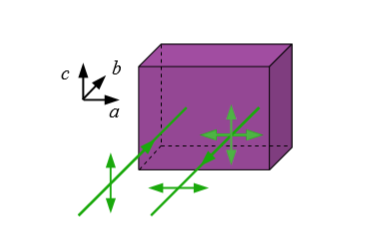
\includegraphics[scale=1]{geometry.PNG}    
\caption{}
\label{Fig:67}
\end{figure}

The following tensors are the example of a point group $$
C_{6 v}, A_{1}
$$ and $$
C_{2 v}, B_{1}
$$ symmetry.

$$
\left(\begin{array}{lll}{a} & {0} & {0} \\ {0} & {a} & {0} \\ {0} & {0} & {b}\end{array}\right) \quad\left(\begin{array}{lll}{0} & {0} & {f} \\ {0} & {0} & {0} \\ {g} & {0} & {0}\end{array}\right)
$$


Here, the zeros represent no phonon modes and the letters shows that the phonon modes are produced. It can be seen that the zeros are always symmetric. Whereas, the same letters represent that the phonon modes are degenerated. \cite{bib1}

\section{Experiment}

This experiment is divided into three parts. Firstly, we needed to do the alignment of the spectrometer. Then the dependence of the linewidth and the width of the entrance slit on the sharpness of the Raman line was observed. Lastly, the Raman spectra for different compounds was determined. 

The alignment was checked by blocking the laser light by mounting all the attenuators in order to protect the CCD from the laser. The spectrometer was moved to $0 cm^{-1}$ relative to the frequency of the laser. The spectrum was observed for a few seconds and then attenuators were removed in order to see the peak around $0 cm^{-1}$. The wavelength was adjusted accordingly in order to see the peak at $0cm^{-1}$.

For the alignment of the Si (111) sample, the attenuator $no.3$ was mounted. The spectrometer was moved to 0 nm in order to align the laser spot on the sample and the sample position. The calibration was done by the alignment camera and the entrance slit was opened. Then, the attenuator was removed in order to observe the laser spot. The entrance slit was varied to get the perfect alignment where the sample is in focus, laser is focused in the center of the sample and the entrance slit. Then, the spectrometer was moved back to around $280 cm^{-1}$ and the mirror was changed back to the CCD mode and the edge filter was mounted. The the spectrum was observed around $520-521 cm^{-1}$. 

The Raman spectra of the samples were observed for all polarization directions. Raman spectra for two polarization direction(horizontal h / Vertical v) can be observed in combination with two polarizations of laser (h/v) which leads to four spectra hh, vv, hv and vh and the last two are equal. \cite{bib1}






\begin{thebibliography}{99}



\bibitem{bib1}
Script, Practical course M 2.8 Raman Spectroscopy. Aug 9,2012

\bibitem{bib2} 
%https://chem.libretexts.org/Bookshelves/Analytical_Chemistry/Map%3A_Principles_of_Instrumental_Analysis_(Skoog_et_al.)/18%3A_Raman_Spectroscopy/18.1%3A_Theory_of_Raman_Spectroscopy





 

\bibitem{} 

\bibitem{} 



\bibitem{} 


\end{thebibliography}






\end{document}

